
\subsubsection{Introduccion}

\subsubsection{Ejercicios}
\begin{itemize}
 \item \textbf{Ejercicio 1 } Programar un tipo de tarea TaskConsola, que simulara una tarea interactiva.
La tarea debe realizar n llamadas bloqueantes, cada una de una duracion al azar 1 entre bmin
y bmax (inclusive). La tarea debe recibir tres parametros: n, bmin y bmax (en ese orden) que
seran interpretados como los tres elementos del vector de enteros que recibe la funcion.
\item \textbf{Ejercicio 2} Escribir un lote de 3 tareas distintas: una intensiva en CPU y las otras dos de
tipo interactivo (TaskConsola). Ejecutar y graficar la simulacion usando el algoritmo FCFS
para 1, 2 y 3 nucleos.
\end{itemize}

Grafico algoritmo FCFS con 1 nucleo.
\vspace*{0.3cm} \vspace*{0.3cm}
  \begin{center}
 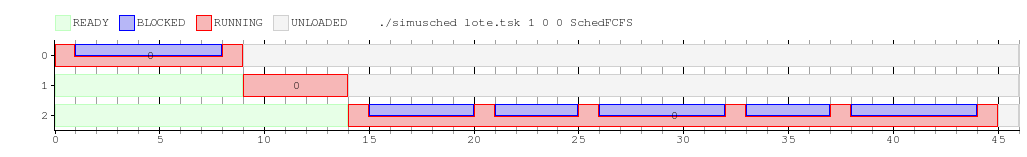
\includegraphics[scale=0.5]{ejercicio2-1nucleo.png}
 \end{center}
  \vspace*{0.3cm}

  Grafico algoritmo FCFS con 2 nucleos.
\vspace*{0.3cm} \vspace*{0.3cm}
  \begin{center}
 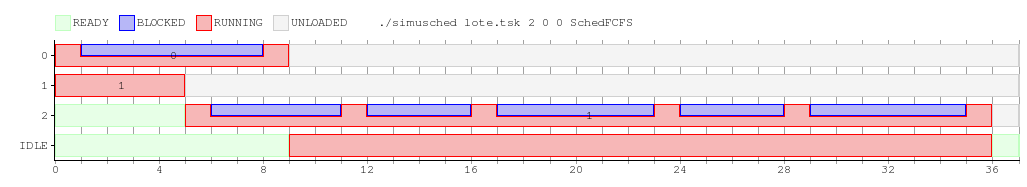
\includegraphics[scale=0.5]{ejercicio2-2nucleo.png}
 \end{center}
  \vspace*{0.3cm}

  Grafico algoritmo FCFS con 3 nucleos.
\vspace*{0.3cm} \vspace*{0.3cm}
  \begin{center}
 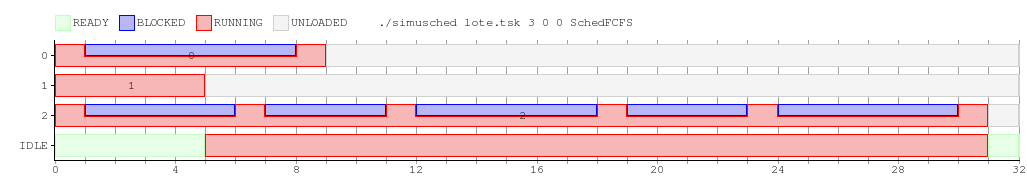
\includegraphics[scale=0.5]{ejercicio2-3nucleo.png}
 \end{center}
  \vspace*{0.3cm}

\indent Debido a las tareas de tipo TaskConsola, se observa que en los tres casos la duración 
de cada bloqueo es distinta.\\
\indent A modo de análisis, se puede observar por medio de los gráficos como aumenta el paralelismo a mayor cantidad de núcleos. 
En este scheduler en particular esto ayuda de gran manera al rendimiento del sistema, puesto que un nucleo podrá ejecutar otra tarea 
recién cuando haya terminado la anterior. Las consecuencias de este comportamiento son visibles en los 3 graficos. Agregando un core más, 
el tiempo que se tarda en ejecutar por completo todas las tareas de reduce casi a la mitad.\\


\subsubsection{Resultados y Conclusiones}

\subsubsection[]{Ejercicio 1}

\begin{verbatim}
 void TaskConsola(int pid, vector<int> params) {
	int i, ciclos;

	for (i = 0; i < params[0]; i++) {
		ciclos = rand() % (params[2] - params[1] + 1) + params[1];
		uso_IO(pid, ciclos);
	}
} 
\end{verbatim}
------------------------------------------------------------------
QUEDA EXPLICAR EL CODIGO
------------------------------------------------------------------
